\begin{frame}{Polygon Decomposition}
\begin{block}{Requirements}
Need a API/framework that 
\begin{itemize}
\item Reads list of points (x,y) and gives output as list-of-lists of points representing sub-polygons 
\item Quiet a few libraries available. Chose '\textbf{Farseer Physics Engine 3.5}. It is a C\# library having many decomposition/triangulation algorithms implemented, along with basic data structures as Vectors, Points etc.
\item Closest to what I needed was Polygon Decomposition by \textbf{Bayazit}
\item Extracted it, removed unnecessary dependencies, changed logic to match decomposition I needed
\item Made a C\#.Net Library (no UI)
\end{itemize}
\end{block}
\end{frame}
%----------------------------------------------------------------------------------------
\begin{frame}{Bayazit Site}
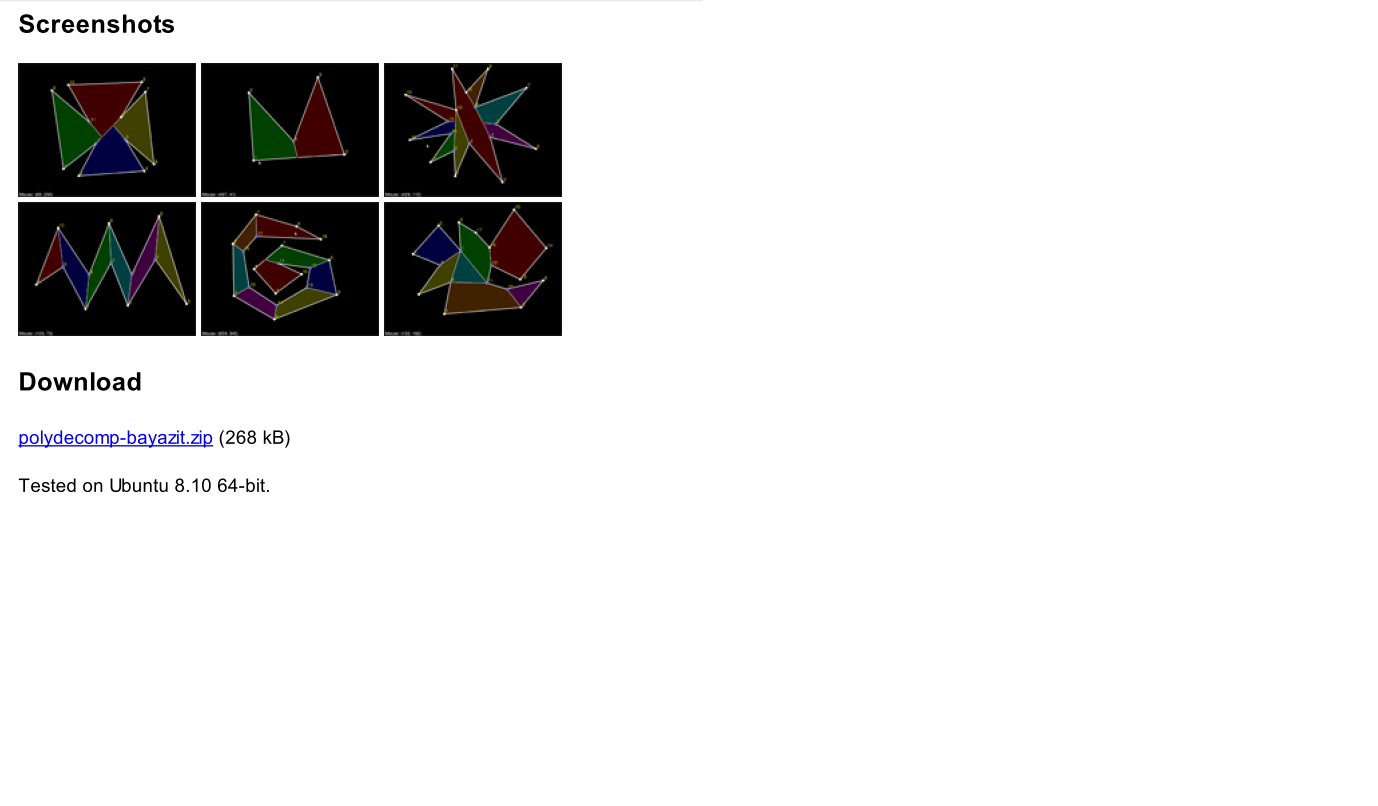
\includegraphics[width=2\linewidth]{../Common/images/ImplBayazitSite.png}
\end{frame}

%-----------------------------------------------------------------------------------------------
\begin{frame}{Midcurves Sample Program}

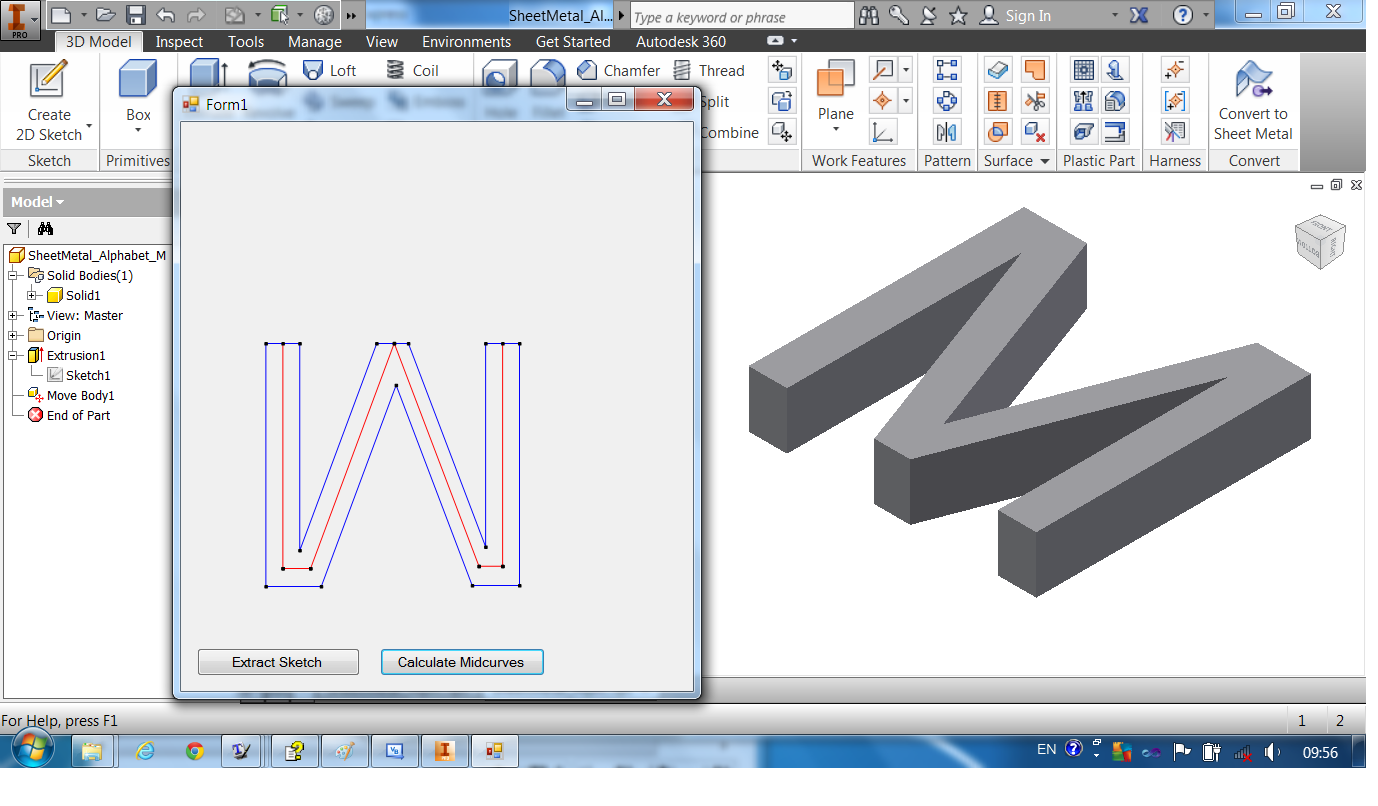
\includegraphics[width=0.9\linewidth]{../Common/images/ImplMidcurvesProgram.png}
\begin{itemize}
\item Load the Part
\item Extract the Sketch, create points list (care has to be taken for Holes)
\item Compute the Midcurve and display results back
\end{itemize}

\end{frame}
